\chapter{3D Phase Tracking Monte Carlo Algorithm}\label{sec:phase}

\section{Introduction}\label{sec:besintro}

\section{Theory}\label{sec:bestheory}

The \gls{mcrt} algorithm as described in~\cref{sec:mcrt}, must be adjusted so that wave phenomena such as interference and diffraction can be modelled. 
Modelling these wave behaviours allows us to model complex beams, where these phenomena are required to form the beam, e.g Bessel beams. 
As \gls{mcrt} is a ballistic simulation of photon packets, meaning that the \gls{mcrt} simulation presented thus far in this thesis only modelled the ballistic behaviour of photons. 
However for the work presented in this chapter, wave like behaviours is crucial to modelling the various experiments and phenomena.

In order to convert a ballistic simulation of photon packets into a ballistic/wave-like simulation, the complex phase of each photon packet is tracked.
This is achieved, by simply tracking the complex phase of the photon as it propagates through a medium.
~\Cref{eqn:phase} shows how the phase is calculated.

\begin{equation}
    \varphi = cos\left(\frac{2 \pi l}{\lambda}\right) + i\ sin\left(\frac{2 \pi l}{\lambda}\right)
    \label{eqn:phase}
\end{equation}

Where $\varphi~[-]$ is the phase of a photon packet, $l\ [m]$ is the distance the photons has travelled, and $\lambda~[m]$ is the wavelength of the photon.
Now we can calculate the phase of a photon at a position $\hat{p_o}$, if we know the distance it has travelled, and its original phase. 
To be able model the wave-like behaviour of photons, we let the photons packets interfere with one another in a volume or area element. 
We do not model the interference at just the points where photons packets cross one another as due to the ballistic nature of the \gls{mcrt} simulation, this does not occur with enough frequency in order to give a good signal to noise ratio. 
The interference takes place in a volume element $dV$ or area element $dA$ instead.
To calculate the interference from the phase, the phase if summed in each volume or area element and the absolute value taken, and then squared, as seen in in~\cref{eqn:intense}.

\begin{equation}
I(\xi)=\left| \sum\limits_{\xi}cos\left(\frac{2\pi d}{\lambda}\right) + i \sum\limits_{\xi}sin\left(\frac{2\pi d}{\lambda}\right)\right|^2,\ \ \ \xi=(x,y,z)
\label{eqn:intense}
\end{equation}

\noindent Where:

\indent $l$ is the total distance travelled by a photon [$m$];

\indent $\lambda$ is the wavelength of the photon [$m$];

\indent $I$ is the intensity at the $\xi^{th}$ cell [dunno].

\medskip

As the \gls{mcrt} simulation is now a quasi ballistic/wave simulation of photon behaviour, we compare our simulations to theoretical and experimental data.

\subsection{Validation of Phase Tracking Algorithm}

The first test of our phase tracking algorithm, is to compare our simulation to a double slit experiment.
The double slit experiment, is a simple experiment where monochromatic plane wave of light is incidence on two slits, and the interference pattern is observed on a screen a distance $d$ away from the slits.
In this experiment


\begin{figure}
\centering
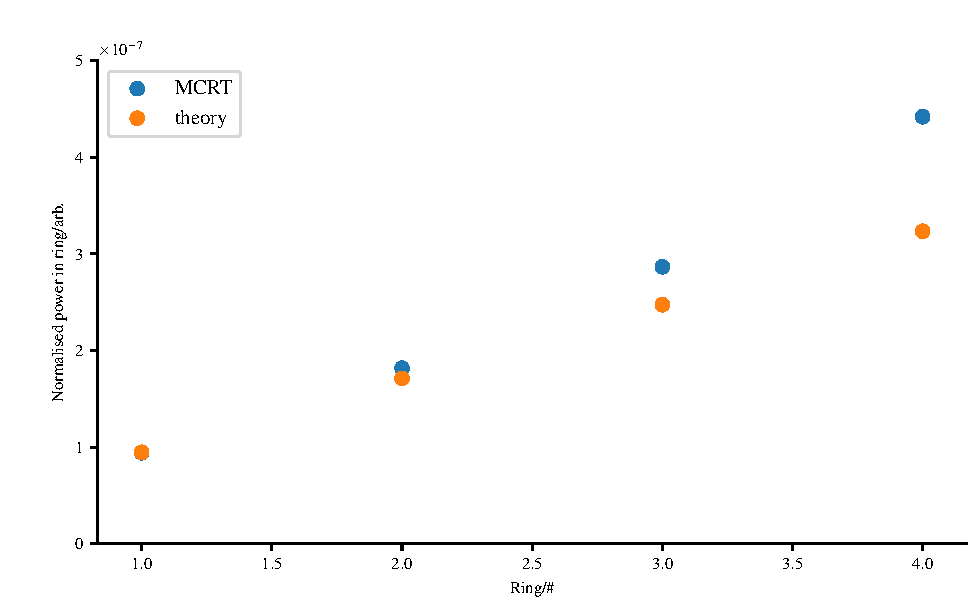
\includegraphics[scale=0.65]{pwr-rings.pdf}
\caption{Bessel beam power in each ring.}
\label{fig:pwrring}
\end{figure}

\begin{figure}
\centering
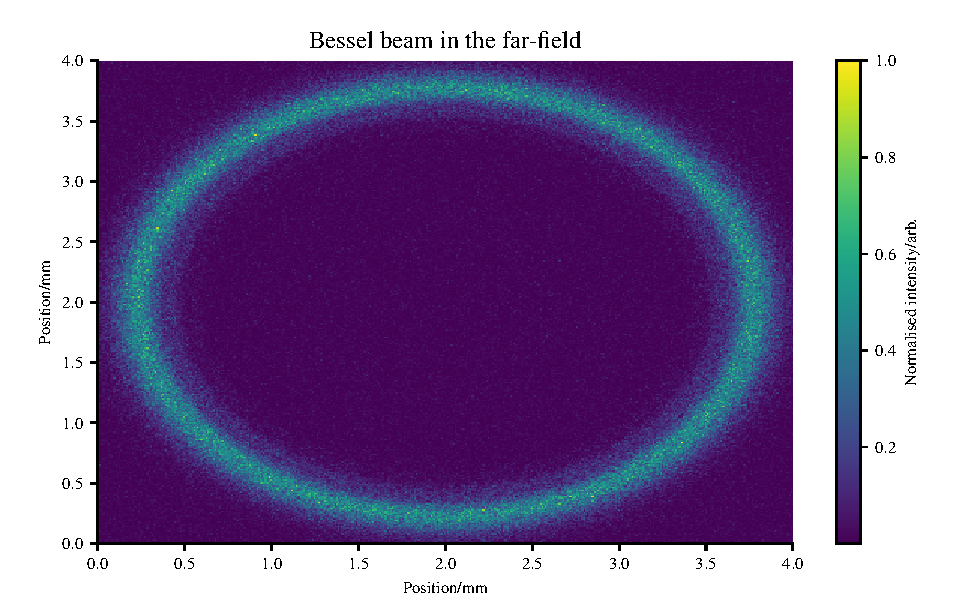
\includegraphics[scale=0.75]{far-field.pdf}
\caption{Bessel beam in the far field.}
\label{fig:farfield}
\end{figure}


a~\cite{mignon2016fractional}
\section{Conclusion}